\documentclass[journal,12pt,twocolumn]{IEEEtran}

\usepackage{setspace}
\usepackage{gensymb}

\singlespacing


\usepackage[cmex10]{amsmath}

\usepackage{amsthm}

\usepackage{mathrsfs}
\usepackage{txfonts}
\usepackage{stfloats}
\usepackage{bm}
\usepackage{cite}
\usepackage{cases}
\usepackage{subfig}

\usepackage{longtable}
\usepackage{multirow}

\usepackage{enumitem}
\usepackage{mathtools}
\usepackage{steinmetz}
\usepackage{tikz}
\usepackage{circuitikz}
\usepackage{verbatim}
\usepackage{tfrupee}
\usepackage[breaklinks=true]{hyperref}
\usepackage{graphicx}
\usepackage{tkz-euclide}
\usepackage{float}

\usetikzlibrary{calc,math}
\usepackage{listings}
    \usepackage{color}                                            %%
    \usepackage{array}                                            %%
    \usepackage{longtable}                                        %%
    \usepackage{calc}                                             %%
    \usepackage{multirow}                                         %%
    \usepackage{hhline}                                           %%
    \usepackage{ifthen}                                           %%
    \usepackage{lscape}     
\usepackage{multicol}
\usepackage{chngcntr}

\DeclareMathOperator*{\Res}{Res}

\renewcommand\thesection{\arabic{section}}
\renewcommand\thesubsection{\thesection.\arabic{subsection}}
\renewcommand\thesubsubsection{\thesubsection.\arabic{subsubsection}}

\renewcommand\thesectiondis{\arabic{section}}
\renewcommand\thesubsectiondis{\thesectiondis.\arabic{subsection}}
\renewcommand\thesubsubsectiondis{\thesubsectiondis.\arabic{subsubsection}}


\hyphenation{op-tical net-works semi-conduc-tor}
\def\inputGnumericTable{}                                 %%

\lstset{
%language=C,
frame=single, 
breaklines=true,
columns=fullflexible
}
\begin{document}
\newtheorem{theorem}{Theorem}[section]
\newtheorem{problem}{Problem}
\newtheorem{proposition}{Proposition}[section]
\newtheorem{lemma}{Lemma}[section]
\newtheorem{corollary}[theorem]{Corollary}
\newtheorem{example}{Example}[section]
\newtheorem{definition}[problem]{Definition}

\newcommand{\BEQA}{\begin{eqnarray}}
\newcommand{\EEQA}{\end{eqnarray}}
\newcommand{\define}{\stackrel{\triangle}{=}}
\bibliographystyle{IEEEtran}
\providecommand{\mbf}{\mathbf}
\providecommand{\pr}[1]{\ensuremath{\Pr\left(#1\right)}}
\providecommand{\qfunc}[1]{\ensuremath{Q\left(#1\right)}}
\providecommand{\sbrak}[1]{\ensuremath{{}\left[#1\right]}}
\providecommand{\lsbrak}[1]{\ensuremath{{}\left[#1\right.}}
\providecommand{\rsbrak}[1]{\ensuremath{{}\left.#1\right]}}
\providecommand{\brak}[1]{\ensuremath{\left(#1\right)}}
\providecommand{\lbrak}[1]{\ensuremath{\left(#1\right.}}
\providecommand{\rbrak}[1]{\ensuremath{\left.#1\right)}}
\providecommand{\cbrak}[1]{\ensuremath{\left\{#1\right\}}}
\providecommand{\lcbrak}[1]{\ensuremath{\left\{#1\right.}}
\providecommand{\rcbrak}[1]{\ensuremath{\left.#1\right\}}}
\theoremstyle{remark}
\newtheorem{rem}{Remark}
\newcommand{\sgn}{\mathop{\mathrm{sgn}}}
\providecommand{\abs}[1]{\vert#1\vert}
\providecommand{\res}[1]{\Res\displaylimits_{#1}} 
\providecommand{\norm}[1]{\lVert#1\rVert}
%\providecommand{\norm}[1]{\lVert#1\rVert}
\providecommand{\mtx}[1]{\mathbf{#1}}
\providecommand{\mean}[1]{E[ #1 ]}
\providecommand{\fourier}{\overset{\mathcal{F}}{ \rightleftharpoons}}
%\providecommand{\hilbert}{\overset{\mathcal{H}}{ \rightleftharpoons}}
\providecommand{\system}{\overset{\mathcal{H}}{ \longleftrightarrow}}
	%\newcommand{\solution}[2]{\textbf{Solution:}{#1}}
\newcommand{\solution}{\noindent \textbf{Solution: }}
\newcommand{\cosec}{\,\text{cosec}\,}
\providecommand{\dec}[2]{\ensuremath{\overset{#1}{\underset{#2}{\gtrless}}}}
\newcommand{\myvec}[1]{\ensuremath{\begin{pmatrix}#1\end{pmatrix}}}
\newcommand{\mydet}[1]{\ensuremath{\begin{vmatrix}#1\end{vmatrix}}}
\numberwithin{equation}{subsection}
\makeatletter
\@addtoreset{figure}{problem}
\makeatother
\let\StandardTheFigure\thefigure
\let\vec\mathbf
\renewcommand{\thefigure}{\theproblem}
\def\putbox#1#2#3{\makebox[0in][l]{\makebox[#1][l]{}\raisebox{\baselineskip}[0in][0in]{\raisebox{#2}[0in][0in]{#3}}}}
     \def\rightbox#1{\makebox[0in][r]{#1}}
     \def\centbox#1{\makebox[0in]{#1}}
     \def\topbox#1{\raisebox{-\baselineskip}[0in][0in]{#1}}
     \def\midbox#1{\raisebox{-0.5\baselineskip}[0in][0in]{#1}}
\vspace{3cm}
\title{ASSIGNMENT 2}
\author{Amulya Tallamraju \\ AI20BTECH11003}
\maketitle
\newpage
\bigskip
\renewcommand{\thefigure}{\theenumi}
\renewcommand{\thetable}{\theenumi}
Download all python codes from 
\begin{lstlisting}
https://github.com/AmulyaTallamraju/EE3900/blob/main/Assignment-3/codes/Assignment-3.py
\end{lstlisting}
%
and latex-tikz codes from 
%
\begin{lstlisting}
https://github.com/AmulyaTallamraju/EE3900/blob/main/Assignment-3/Assignment-3.tex
\end{lstlisting}
\section{Construction 2.10}
Construct a quadrilateral MORE where $MO = 6, OR = 4.5, \angle M = 60 \degree, \angle O = 105 \degree$ and $\angle R = 105 \degree$.
%
\section{SOLUTION}
Given
    \begin{align}
    &\angle M= 60\degree=\theta \label{eq1}
    \\
    &\angle O= 105\degree=\alpha
    \\
    &\angle R= 105\degree=\delta \label{eq2}
    \\
    &\norm{\vec{O}-\vec{M}} =6=a, \label{eq3}
    \\
    &\norm{\vec{R}-\vec{O}} =4.5=b,\label{eq4}
    \\
    &\vec{M}=\myvec{0\\0}, \vec{O}=\myvec{6\\0}
    \end{align}
      Let
\begin{align}
 &\norm{\vec{R}-\vec{E}}=c
 \\
  &\norm{\vec{M}-\vec{E}} =d 
  \\
    &\norm{\vec{M}-\vec{R}} =e
  \\
  &\theta= \theta_1 + \theta_2
  \\
  & \delta_1=\angle ERM \\
  & \delta_2= \angle ORM\\
  & \gamma= \angle E
\end{align}
\begin{lemma}
If three angles and two sides of a quadrilateral are known, then the coordinates of the vertices can be expressed as
\begin{align}
    \vec{R}=\vec{O}+b\times \myvec{\cos \alpha \\ \sin \alpha}\\
    \vec{E}=d \myvec{\cos \theta \\ \sin \theta}
\end{align}
where 
\begin{align}
    d=e \times \brak{\frac{\sin\brak{{\delta-\sin^{-1}\sbrak{\sin{\alpha}\times \brak{\frac{b}{e}}}}}}{\sin\brak{{360\degree-(\alpha+\theta+\delta)}}}}
\times
\end{align}
and
\begin{align}
    e=\sqrt{a^2+b^2-2\times a \times b\cos{\alpha}}
\end{align}
\end{lemma}
\begin{proof}
\begin{align}
\gamma=360\degree-(\alpha+\theta+\delta)
\end{align}
 Now, using cosine formula in $\triangle MOR$ we can find e:
\begin{align}
 e^2=
a^2+b^2-2\times a \times b\cos{\alpha}
\end{align}
Using sine rule,
\begin{align}
    \frac{\sin{\alpha}}{e}=\frac{\sin{\delta_2}}{b}\\
    \delta_2=\sin^{-1}\sbrak{\sin{\alpha}\times \brak{\frac{b}{e}}}\\
\end{align}
  Now in $\triangle MER$,
  \begin{align}
  \delta_1=\delta-\delta_2
  \end{align}
Using sine law of triangle,
\begin{align}
    \frac{\sin{\gamma}}{e}&=\frac{\sin{\delta_1}}{d}\\
    \implies d&=e\times \brak{\frac{\sin{\delta_1}}{\sin{\gamma}}}
\end{align}
From the above equations, we get
\begin{align}
d=e \times \brak{\frac{\sin\brak{{\delta-\sin^{-1}\sbrak{\sin{\alpha}\times \brak{\frac{b}{e}}}}}}{\sin\brak{{360\degree-(\alpha+\theta+\delta)}}}}
\times 
\end{align}
where
\begin{align}
    e=\sqrt{a^2+b^2-2\times a \times b\cos{\alpha}}
\end{align}
\end{proof}
  Calculating the co-ordinates of $\vec{R}$:\\
 Putting the values in the above equation we get,
 \begin{align}
     \implies \vec{R}= \myvec{6\\0}+4.5 \myvec{\cos 105\degree\\ \sin 105\degree}
 \end{align}
 \begin{align}
     \implies \vec{R}= \myvec{6\\0}+\myvec{1.16\\4.35}
 \end{align}
 \begin{align}
     \vec{R}= \myvec{7.16\\4.35}
 \end{align}
       Calculating the co-ordinates of $\vec{E}$:\\
 Putting the values in the above equation we get,
 \begin{align}
     \implies \vec{E}= 7.34 \myvec{\cos 60\\ \sin 60}
 \end{align}
 \begin{align}
     \implies \vec{E}= \myvec{3.67\\6.36}
 \end{align}
   Now, we have the coordinate of vertices M,O,R,E as,
\begin{align}
\vec{M}= \myvec{0 \\ 0}, \vec{O}= \myvec{6 \\ 0},  \vec{R}= \myvec{7.16 \\ 4.35}, \vec{E}= \myvec{3.67 \\ 6.36}.
\end{align}    
      On constructing the given quadrilateral on python  we get:
\begin{figure}[!ht]
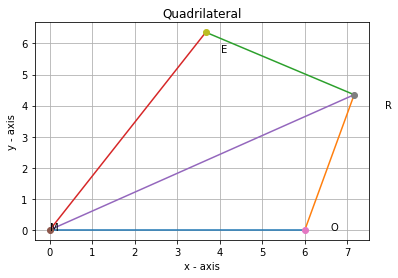
\includegraphics[ width=\columnwidth, height=6 cm]{quad.png}
\caption{Quadrilateral MORE}
\label{fig:Quadrilateral MORE}	
\end{figure}
\end{document}